\documentclass[10pt, letterpaper]{article}
\usepackage{amsmath}
\usepackage{amssymb}
\usepackage{graphicx}
\usepackage{caption}
\captionsetup{justification=raggedright, singlelinecheck=false, labelfont=bf}
\usepackage[backend=bibtex, style=authoryear]{biblatex}
% \usepackage{wrapfig}
\usepackage{tikz}
% \usepackage{pgfplots}
\usetikzlibrary{shapes.geometric}
\usetikzlibrary{positioning}
\usetikzlibrary{arrows, decorations.pathreplacing}

\addbibresource{refs.bib}

% \addbibresource{~/Dropbox/checkoffGrantProposal/checkoffGrantRef.bib}
\AtBeginBibliography{\small}
\usepackage{xcolor}
\definecolor{hyperblue}{rgb}{0,0,0.4}

\usepackage[noindentafter]{titlesec}

\titleformat*{\section}{\large\bfseries}
\titleformat*{\subsection}{\normalsize\bfseries}
\titleformat*{\subsubsection}{\small\bfseries}

\graphicspath{{plots/}}

% for commenting
\usepackage[mmddyyyy,hhmmss]{datetime}
\usepackage{xcolor}

\definecolor{nicholasCol}{RGB}{203,97,63}
\definecolor{kellyCol}{RGB}{0,50,200}

\newcommand{\nicholas}[1]{{\color{nicholasCol} [\textbf{NS:} #1 (\today\ \currenttime)]}}
\newcommand{\kelly}[1]{{\color{kellyCol} [KR: #1 (\today\ \currenttime)]}}



% \titlespacing{command}{left spacing}{before spacing}{after spacing}[right]
% spacing: how to read {12pt plus 4pt minus 2pt}
%           12pt is what we would like the spacing to be
%           plus 4pt means that TeX can stretch it by at most 4pt
%           minus 2pt means that TeX can shrink it by at most 2pt
%       This is one example of the concept of, 'glue', in TeX

\titlespacing\section{0pt}{12pt plus 4pt minus 2pt}{0pt plus 2pt minus 2pt}
\titlespacing\subsection{0pt}{12pt plus 4pt minus 2pt}{0pt plus 2pt minus 2pt}
\titlespacing\subsubsection{0pt}{12pt plus 4pt minus 2pt}{0pt plus 2pt minus 2pt}


\usepackage{hyperref}[hidelinks]

\hypersetup{
	colorlinks = true, %Colours links instead of ugly boxes
	urlcolor = hyperblue, %Colour for external hyperlinks
	linkcolor = hyperblue, %Colour of internal links
    anchorcolor = hyperblue,
    citecolor = hyperblue,
    filecolor = hyperblue,
     }

\usepackage[margin=0.7in]{geometry}
% \textwidth=470pt
% \oddsidemargin=0pt
% \topmargin=0pt
% \headheight=0pt
% \textheight=660pt
% \headsep=0pt

\setlength{\parskip}{0.2\baselineskip}%



% \title{Sequencing alfalfa populations to evaluate genome-wide prediction of forage growth curves. 
% }


\author{Nicholas Santantonio}
\date{\today}


\newcommand{\GxE}{G$\times$E}
\newcommand{\GxG}{G$\times$G}

\renewcommand{\topfraction}{0.7}  % max fraction of floats at top
\renewcommand{\floatpagefraction}{0.7}% max fraction of page used for floats
\renewcommand{\textfraction}{.2} % minimum fraction of page used for text

\begin{document}

\noindent  \LARGE{\textbf{NAFA: U.S. Alfalfa Farmer Research Initiative - Checkoff}}

\noindent \Large{\textbf{Title:} \textit{Evaluating approaches to high-throughput phenotyping and genotyping for genomic selection in alfalfa}} \hfill \normalsize{\textbf{PI:} Kelly Robbins, Cornell University, (607) 255-8819, \texttt{krr73@cornell.edu}} \\


% \noindent \textbf{PI:} Kelly Robbins$^1$, \textbf{Co-PI:} Don Viands$^1$, \textbf{Co-PI:} Julie Hansen$^1$, \textbf{Author:} Nicholas Santantonio$^2$  \\
% \noindent $^1$Plant Breeding and Genetics Section, School of Integrated Plant Sciences, College of Agriculture and Life Sciences, Cornell University, Ithaca NY.\\
% \noindent $^2$School of Plant and Environmental Sciences, College of Agriculture and Life Sciences, Virginia Tech, Blacksburg VA.


% Address
% Phone:
% Fax:
% Email:


\begin{minipage}{0.5\linewidth}%
\large{\textbf{Objectives \& Motivation}}
\raggedright{
\noindent \begin{itemize}
	\item Develop a genotyping approach to estimate genetic relationships between alfalfa populations, which are not genetically distinct individuals
	\begin{itemize}
		\item Population-level sequence-based genotyping to estimate population allele frequencies
		\item Use pairwise $F{st}$ to estimate additive covariance between populations
	\end{itemize}
	\item Incorporate aerial high-throughput phenotyping to predict performance and genetic merit of breeding materials
	\begin{itemize}
		\item Predict population performance using genetic relationships and vegetative indices
		\item Longitudinal random regression to estimate genotype-specific growth curves
	\end{itemize}
	% \rule{\linewidth}{}

\end{itemize}
}
\end{minipage}%
\begin{minipage}{0.05\linewidth}
\
\end{minipage}%
\begin{minipage}{0.45\linewidth}
% \raggedright
% \centering
\begin{tabular*}{\hsize}{@{\extracolsep{\fill}}lcrr}
% \begin{tabular}{lrrr}
  % \hline
 Harvest & Year & $F_{st}$ & covAF \\ 
  \hline
  2 & 2019 & 0.27 & 0.43 \\ 
  3 & 2019 & 0.75 & 0.73 \\ 
  1 & 2020 & 0.51 & 0.24 \\ 
  2 & 2020 & 0.94 & 0.97 \\ 
  Sum of 4 harvests & - & 0.90 & 0.79 \\ 
   \hline
\end{tabular*}
\smallskip

\textbf{Table 1:} Leave one out genomic prediction accuracy for genetic covariances estimated by pairwise $F_{st}$ or covariance of allele frequencies (covAF) of eight Cornell populations evaluated in Geneva, NY.

\bigskip
\large{\textbf{Study Design and Materials}}
\raggedright{
\noindent \begin{itemize}
	\item Diallel of 9 alfalfa germplasm sources \parencite{segovia2004}
	\begin{itemize}
		\item 9 parental, 36 hybrid populations
		\item Forage yield 1997, 1998
	\end{itemize}
	\item Eight Cornell varieties and breeding populations
	\begin{itemize}
		\item Imaged (NDVI) every $\sim 4.3$ days
		\item 4 harvests across 2019 and 2020
	\end{itemize}
\end{itemize}
}
\end{minipage}%

\begin{minipage}{0.6\linewidth}%
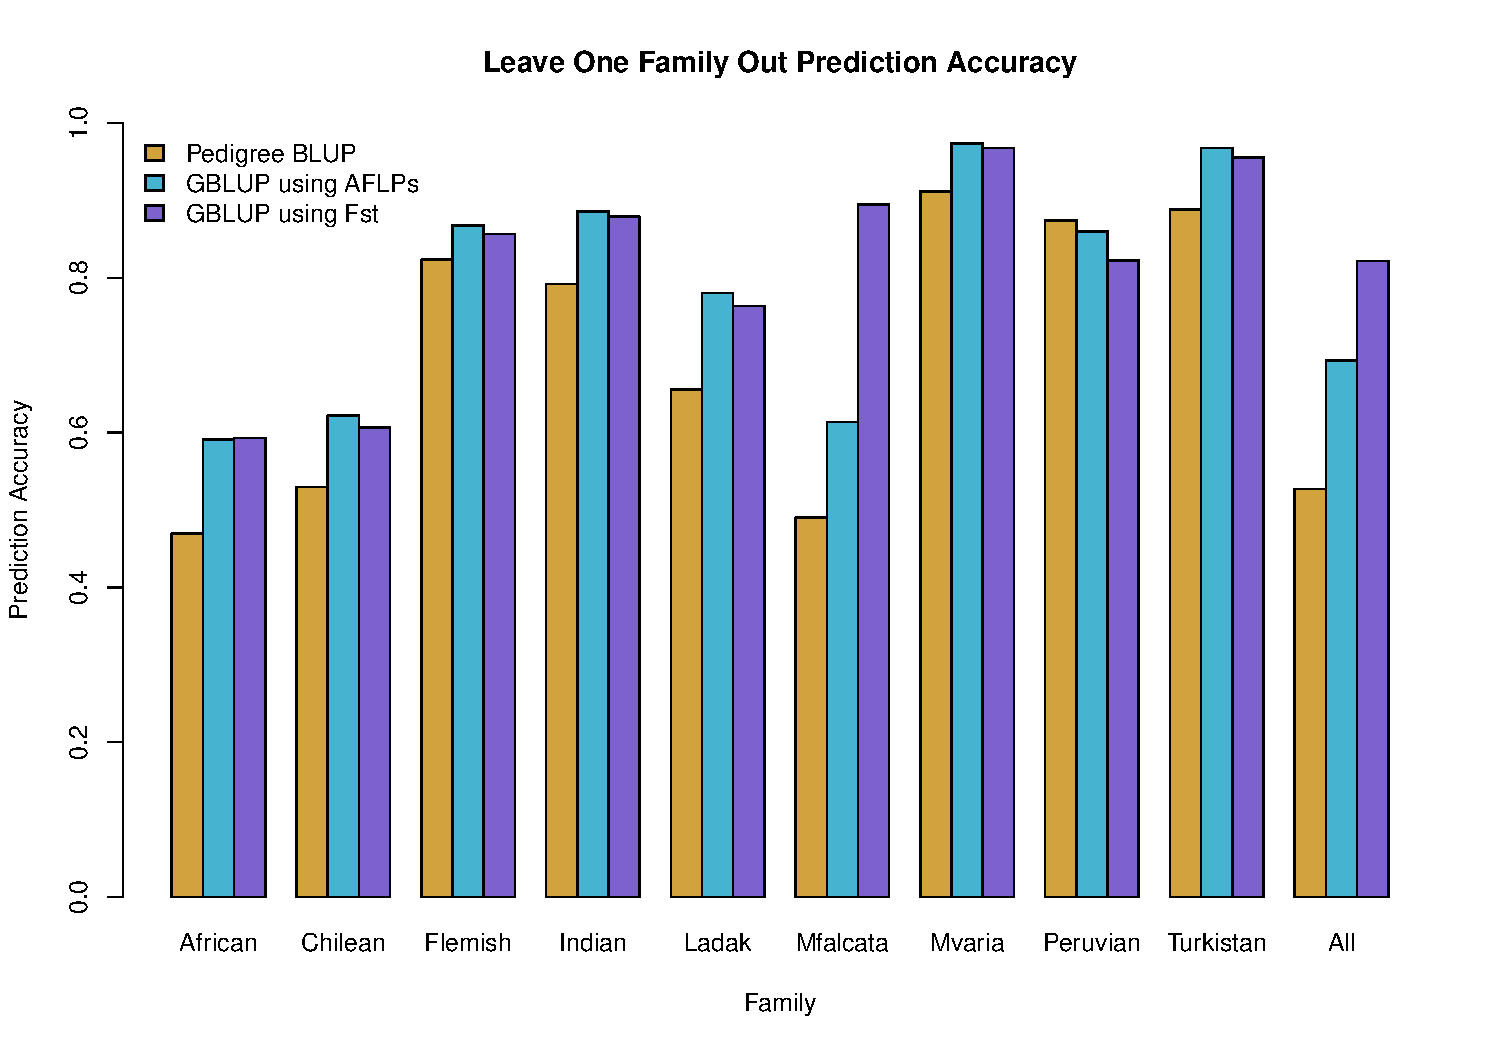
\includegraphics[width = \linewidth]{FstLeaveOneFamOutPredAcc} \\
\textbf{Figure 1:} Prediction accuracy using a leave one family out strategy for a diallel population with 9 parental populations, and 36 hybrid populations of alfalfa. For each of the nine parents, all entries with that parent were removed and predicted using the remaining eight families and the additive genetic covariance estimated using pedigrees, dominant markers \parencite[1544 AFLPs;][]{segovia2003}, or $F_{st}$ statistics calculated from variant frequencies determined by whole-genome resequencing.
\end{minipage}%
\begin{minipage}{0.05\linewidth}
\
\end{minipage}%
\begin{minipage}{0.35\linewidth}

\large{\textbf{Results}}
\raggedright{
\noindent \begin{itemize}
	\item $F_{st}$ increased accuracy over dominant markers
	\item Variable prediction with single NDVI time points
	\item Growth curves incorporate many time points, highly related to forage yield and quality 

\end{itemize}
}

\large{\textbf{Data Availability}}\\
Images processed and stored on \href{https://www.imagebreed.org/}{Imagebreed} online database \parencite{morales2020}

\vspace{5mm}
\large{\textbf{Acknowledgments}}\\
Noble Research Institute for providing the tetraploid alfalfa genome assembly (collaborator: Dr. Maria Monteros).

\end{minipage}%

% \includegraphics[width = \linewidth]{"\string~/Dropbox/checkoffUpdate2020/Fig2USAFRIupdate"}


% \newpage

\hspace{-0.5cm}
 \begin{tikzpicture}

 \begin{scope}[xshift=-6cm, yshift=6cm, scale=0.3]
    \node () at (0,0) {\textbf{Growth curve deviations}};
  \end{scope}

\begin{scope}[xshift=0cm, yshift=6cm, scale=0.3]
    \node () at (0,0) {\textbf{Growth curves}};
  \end{scope}

\begin{scope}[xshift=6cm, yshift=6.2cm, scale=0.3]
    \node () at (0,0) {\begin{tabular}{c} \textbf{Area under the} \\ \textbf{growth curve (AUGC)} \end{tabular}};
  \end{scope}
%%%%%%%%%%%%%%%%%%
\begin{scope}[xshift=-9.1cm, yshift=3cm, scale=0.3]
    \node[rotate = 90] () at (0,0) {\textbf{Harvest 3, 2019}};
  \end{scope}

\begin{scope}[xshift=-9.1cm, yshift=-3cm, scale=0.3]
    \node[rotate = 90] () at (0,0) {\textbf{Harvest 2, 2020}};
  \end{scope}

%%%%%%%%%%%

  \begin{scope}[xshift=-6cm, yshift=3cm, scale=0.3]
    \node () at (0,0) {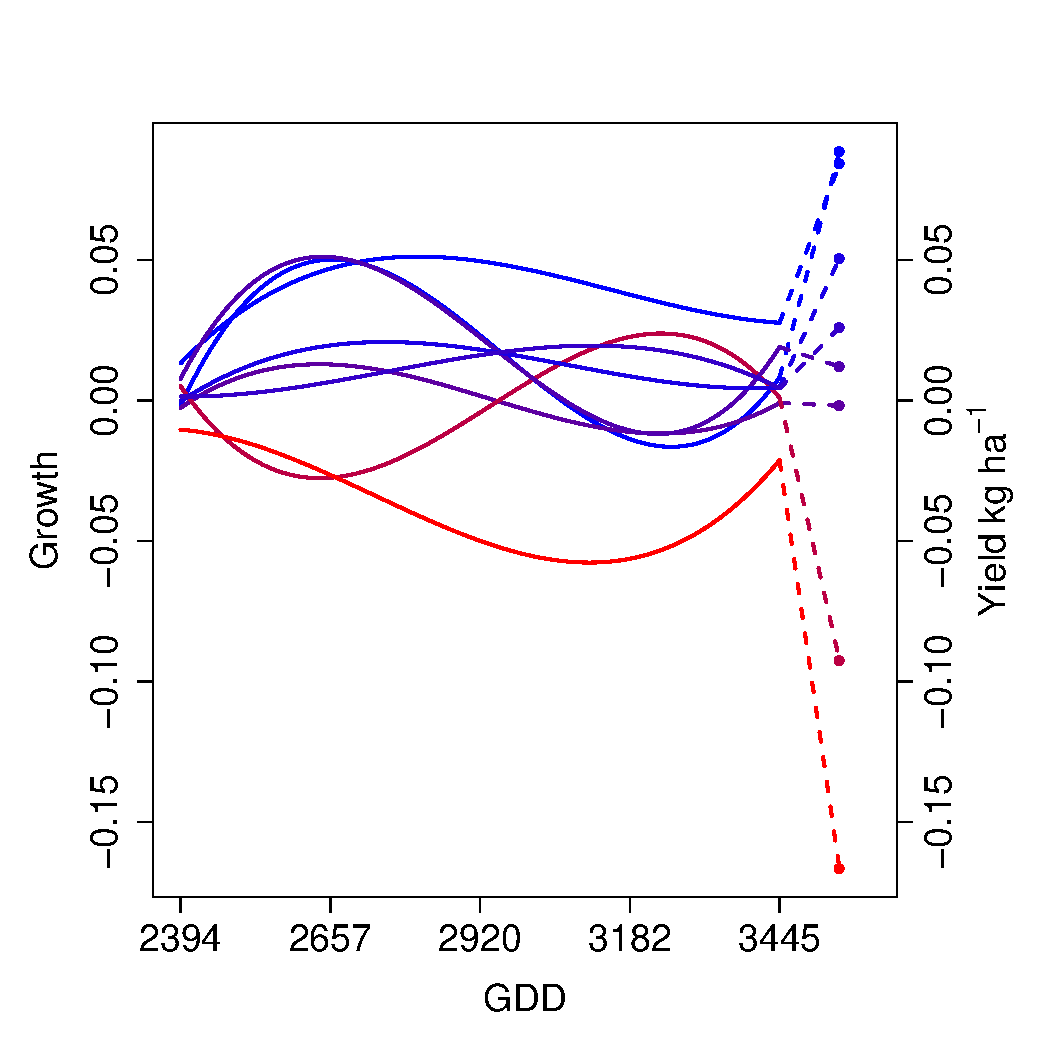
\includegraphics[width = 6cm]{growthCurveDeviations_ndvi_yld_h3_2019_geno8}};
  \end{scope}

  \begin{scope}[xshift=0cm, yshift=3cm, scale=0.3]
    \node () at (0,0) {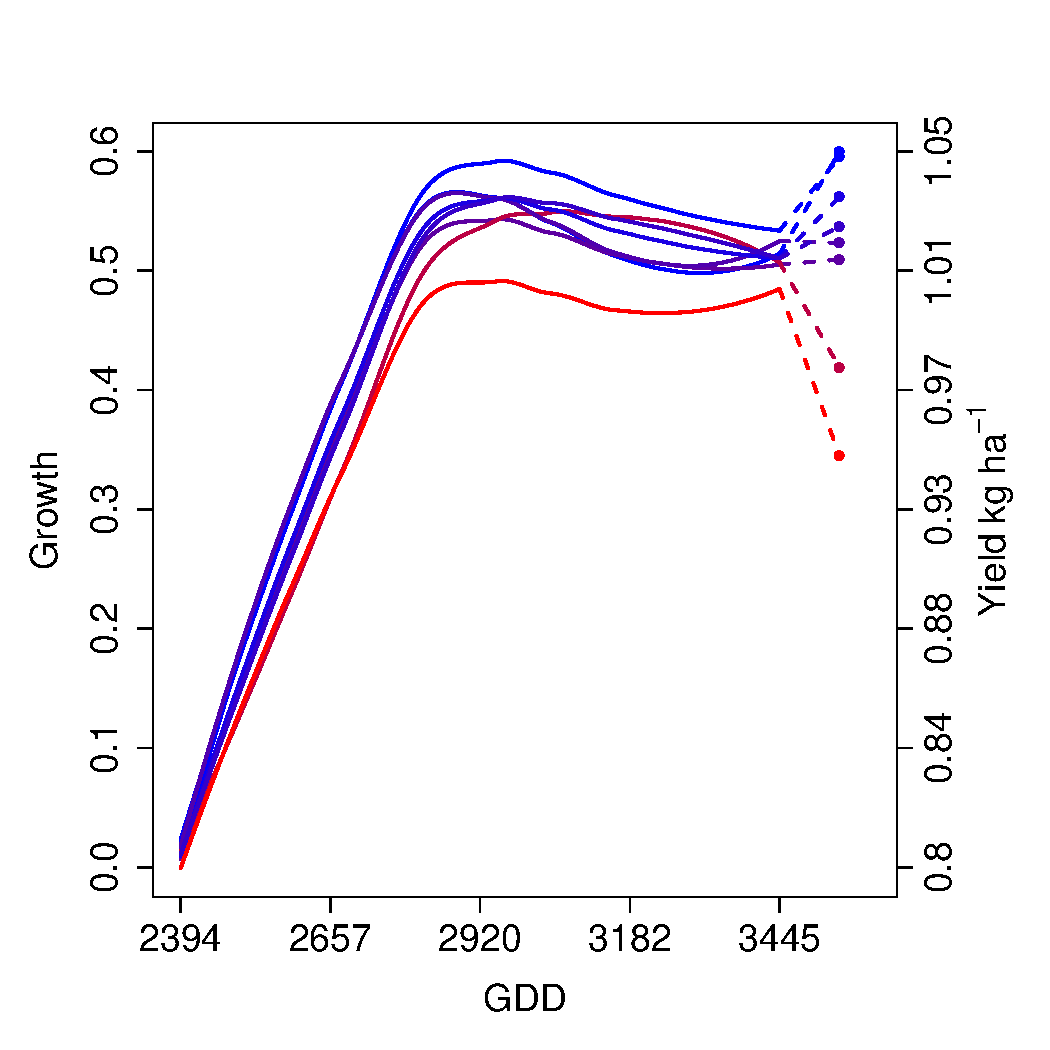
\includegraphics[width = 6cm]{growthCurvesWithMeanCurve_ndvi_yld_h3_2019_geno8}};
  \end{scope}

  \begin{scope}[xshift=6cm, yshift=3cm, scale=0.3]
    \node () at (0,0) {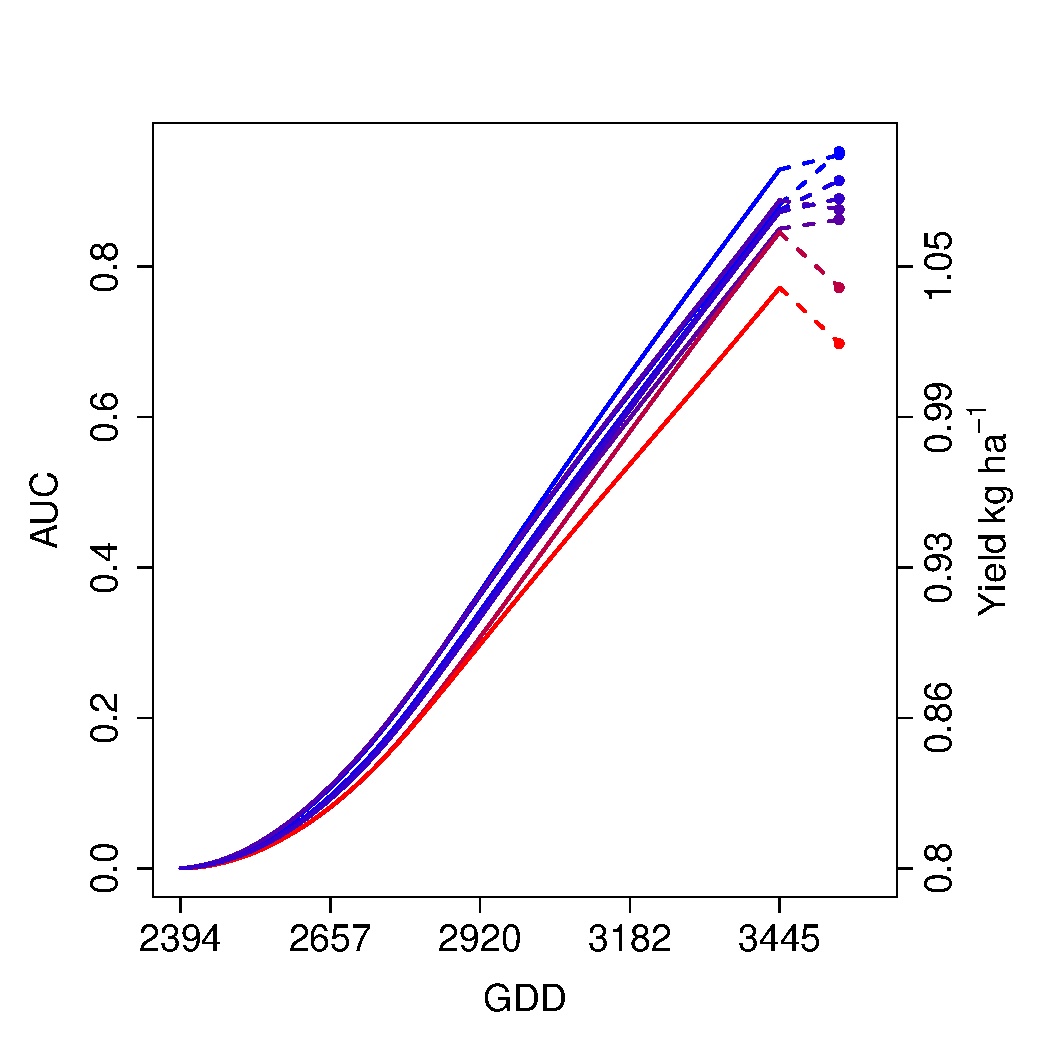
\includegraphics[width = 6cm]{AUC_ndvi_yld_h3_2019_geno8}};
  \end{scope}

  \begin{scope}[xshift=-6cm, yshift=-3cm, scale=0.3]
    \node () at (0,0) {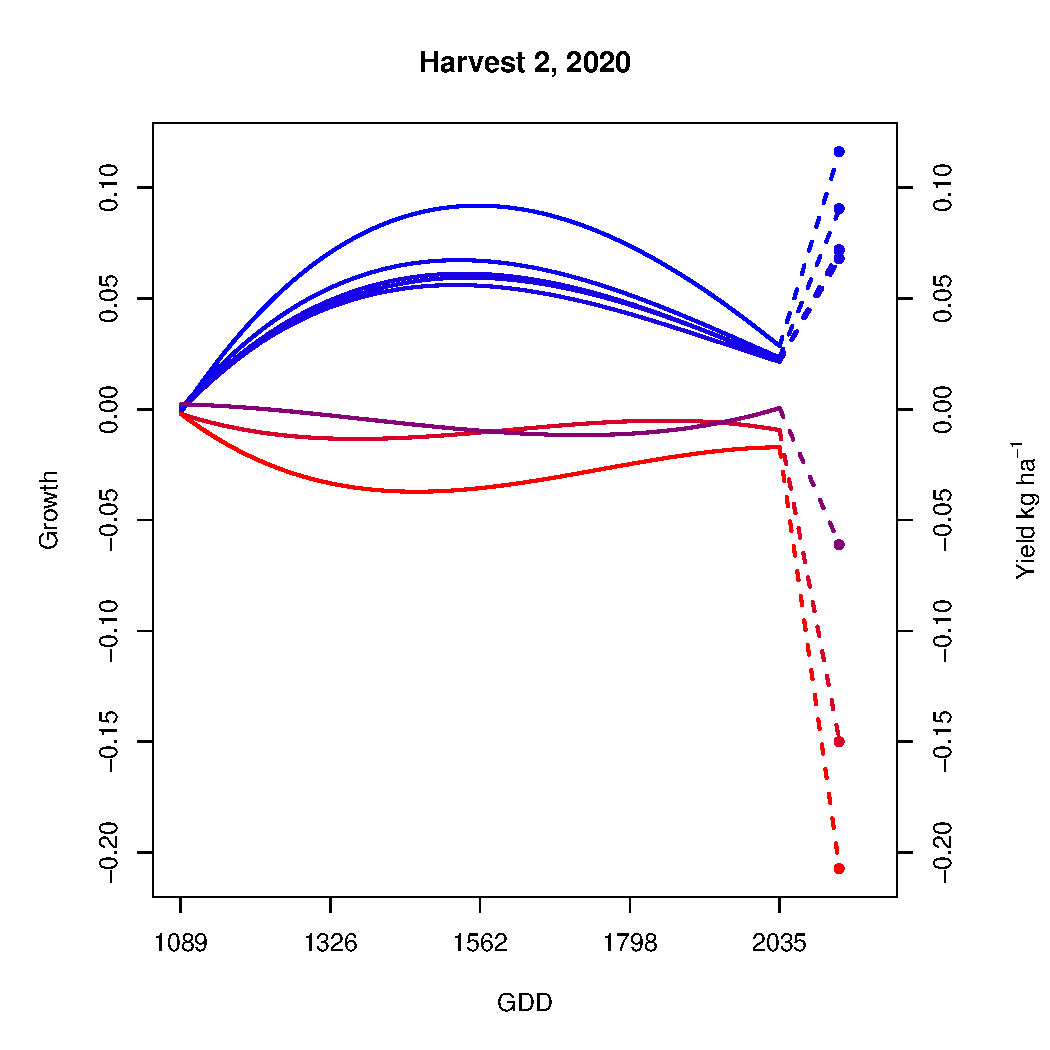
\includegraphics[width = 6cm]{growthCurveDeviations_ndvi_yld_h2_2020_geno8}};
  \end{scope}

  \begin{scope}[xshift=0cm, yshift=-3cm, scale=0.3]
    \node () at (0,0) {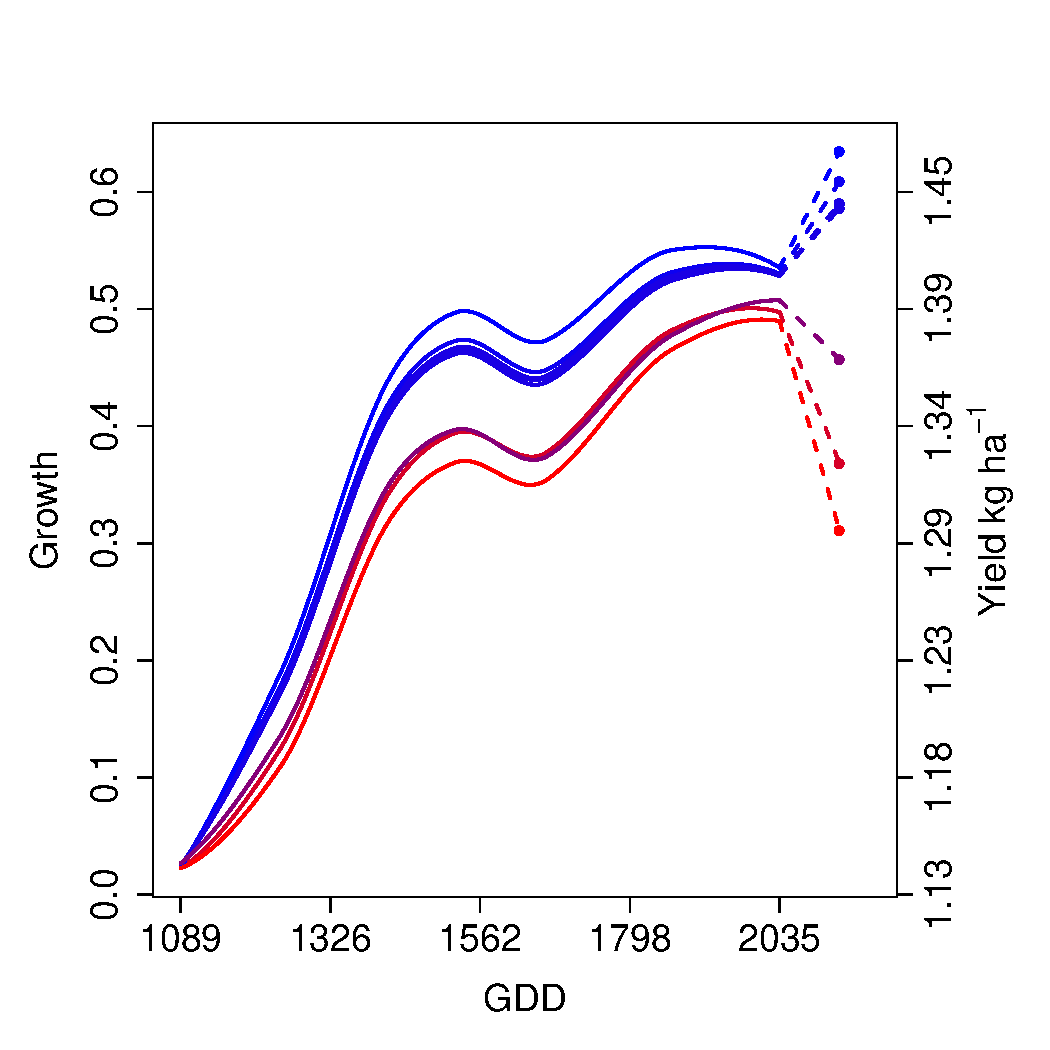
\includegraphics[width = 6cm]{growthCurvesWithMeanCurve_ndvi_yld_h2_2020_geno8}};
  \end{scope}

  \begin{scope}[xshift=6cm, yshift=-3cm, scale=0.3]
    \node () at (0,0) {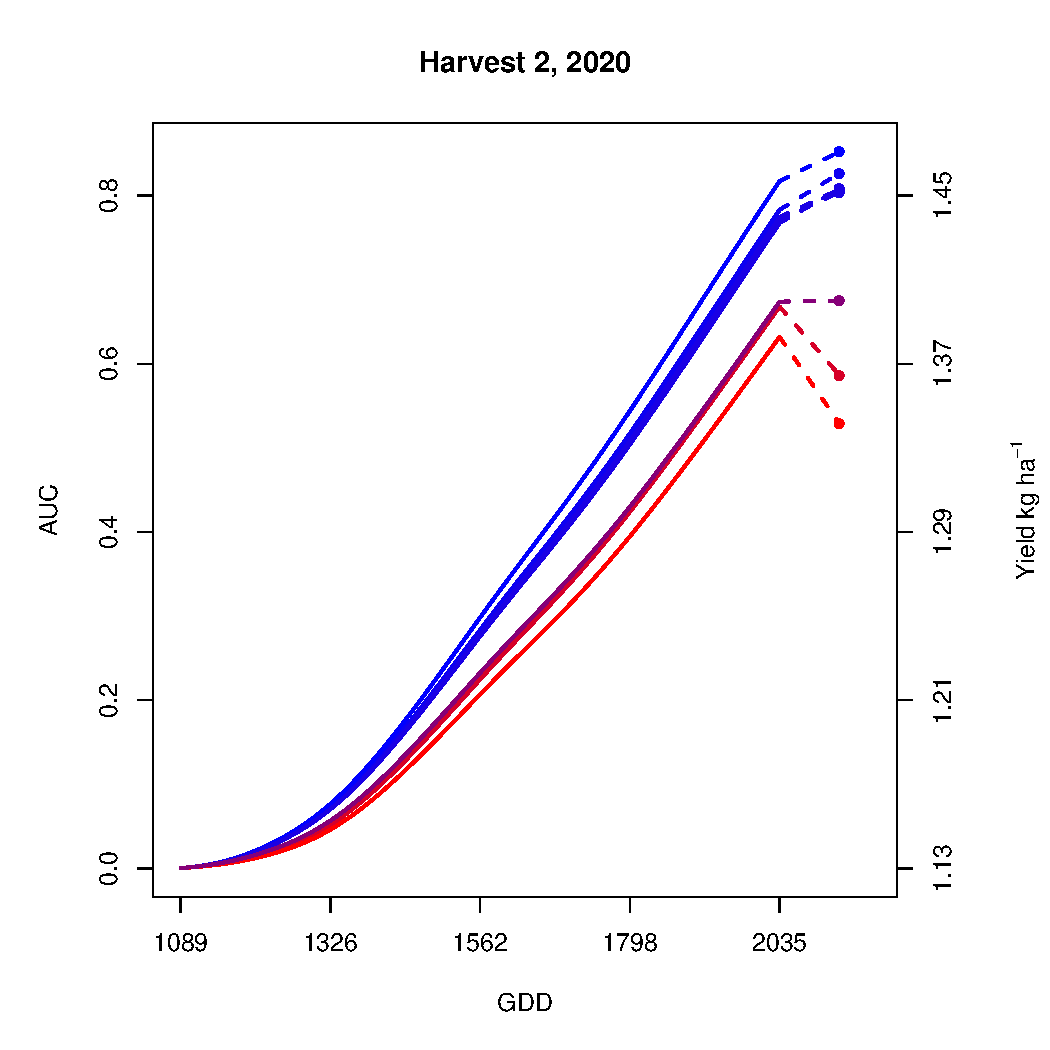
\includegraphics[width = 6cm]{AUC_ndvi_yld_h2_2020_geno8}};
  \end{scope}

 \end{tikzpicture}\\
\textbf{Figure 2:} Genetic growth curve deviations are the genetic differences from a mean genetic curve estimated in a longitudinal random regression using Legendre polynomials. Genetic growth curves have the mean growth curve added back in. The area under the genetic growth curve estimates the accumulation and partitioning of photosynthate to forage yield (FY) in two harvests in 2019 and 2020. Blue = high FY, Red = low FY.

\medskip

\noindent \rule{\linewidth}{0.1pt}

\medskip


\noindent%
\begin{minipage}[h]{.45\textwidth}
\centering
\textbf{ Forage Yield Harvest 3, 2019}

\medskip
\begin{tabular}{rrrrrr}
  % \hline
 & L0 & L1 & L2 & L3 & FY \\ 
  \hline
  L0 &  & 0.04 & -0.91 & 0.12 & 0.81 \\ 
  L1 & &  & -0.04 & -0.98 & -0.15 \\ 
  L2 & & &  & -0.11 & -0.95 \\ 
  L3 & & & &  & 0.28 \\ 
   \hline
\end{tabular}
\end{minipage}%
\begin{minipage}[h]{.05\textwidth}
\
\end{minipage}%
\begin{minipage}[h]{.45\textwidth}
\centering
\textbf{Forage Yield Harvest 2, 2020}

\medskip
\begin{tabular}{rrrrrr}
  % \hline
 & L0 & L1 & L2 & L3 & FY \\ 
  \hline
  L0 &   & 0.54 & -0.99 & 0.72 & 0.95 \\ 
  L1 & &   & -0.55 & -0.09 & 0.36 \\ 
  L2 & & &   & -0.66 & -0.91 \\ 
  L3 & & & &   & 0.87 \\ 
   \hline
\end{tabular}
\end{minipage}% <---------------- Note the use of "%"

\smallskip

\noindent \textbf{Table 2:} Genetic correlations of Legendre polynomial parameters, L0, L1, L2, and L3 with forage yield (FY) in two harvests in 2019 and 2020. Intercepts ($L0$) were high correlated to forage yield(FY), while quadratic terms were highly negatively correlated with FY.

% \smallskip

\noindent \rule{\linewidth}{0.1pt}
\smallskip

\large
\noindent%
\begin{minipage}[h]{.475\textwidth}
\textbf{Conclusions:}
\begin{enumerate}
	%   \setlength\itemsep{0.2em}
	% \item Evaluate the efficacy of using a sequence-based population-level bulk genotyping approach to predict yield performance in diverse and elite germplasm.%
	% \item Estimate the genetic correlations of multi-spectral indices with forage yield and quality using population-level genomic relationships.%
	% \item Determine efficacy of phenotype reduction using spectral indices.%
	% \item Fit population specific growth curves for each harvest using genomic relationships and spectral indices.% 
	\item Pairwise $F_{st}$ values serve as efficient estimates of genetic relatedness between populations.%
	\item Genetic correlations between forage yield and vegetative indices are high, especially in first half of regrowth period.%
\end{enumerate}%
\end{minipage}% <---------------- Note the use of "%"
\begin{minipage}[h]{.05\textwidth}
\quad
\end{minipage}
\begin{minipage}[h]{.475\textwidth}
\vspace{1mm}
\begin{enumerate}
	  \setlength\itemsep{0.2em}
	  \setcounter{enumi}{2}
	\item Vegetative indices were predictive of forage yield and quality, but including genetic covariance was more important.%
	\item Early growth tends to lead to higher forage yields, but with lower quality. Quality reduction likely related to maturity.%
\end{enumerate}%
\end{minipage}

\smallskip

\end{document}
